\subsection{Audio Deepfake Detection Service}

\begin{figure}[H]
    \vspace{1em}
    \centering
    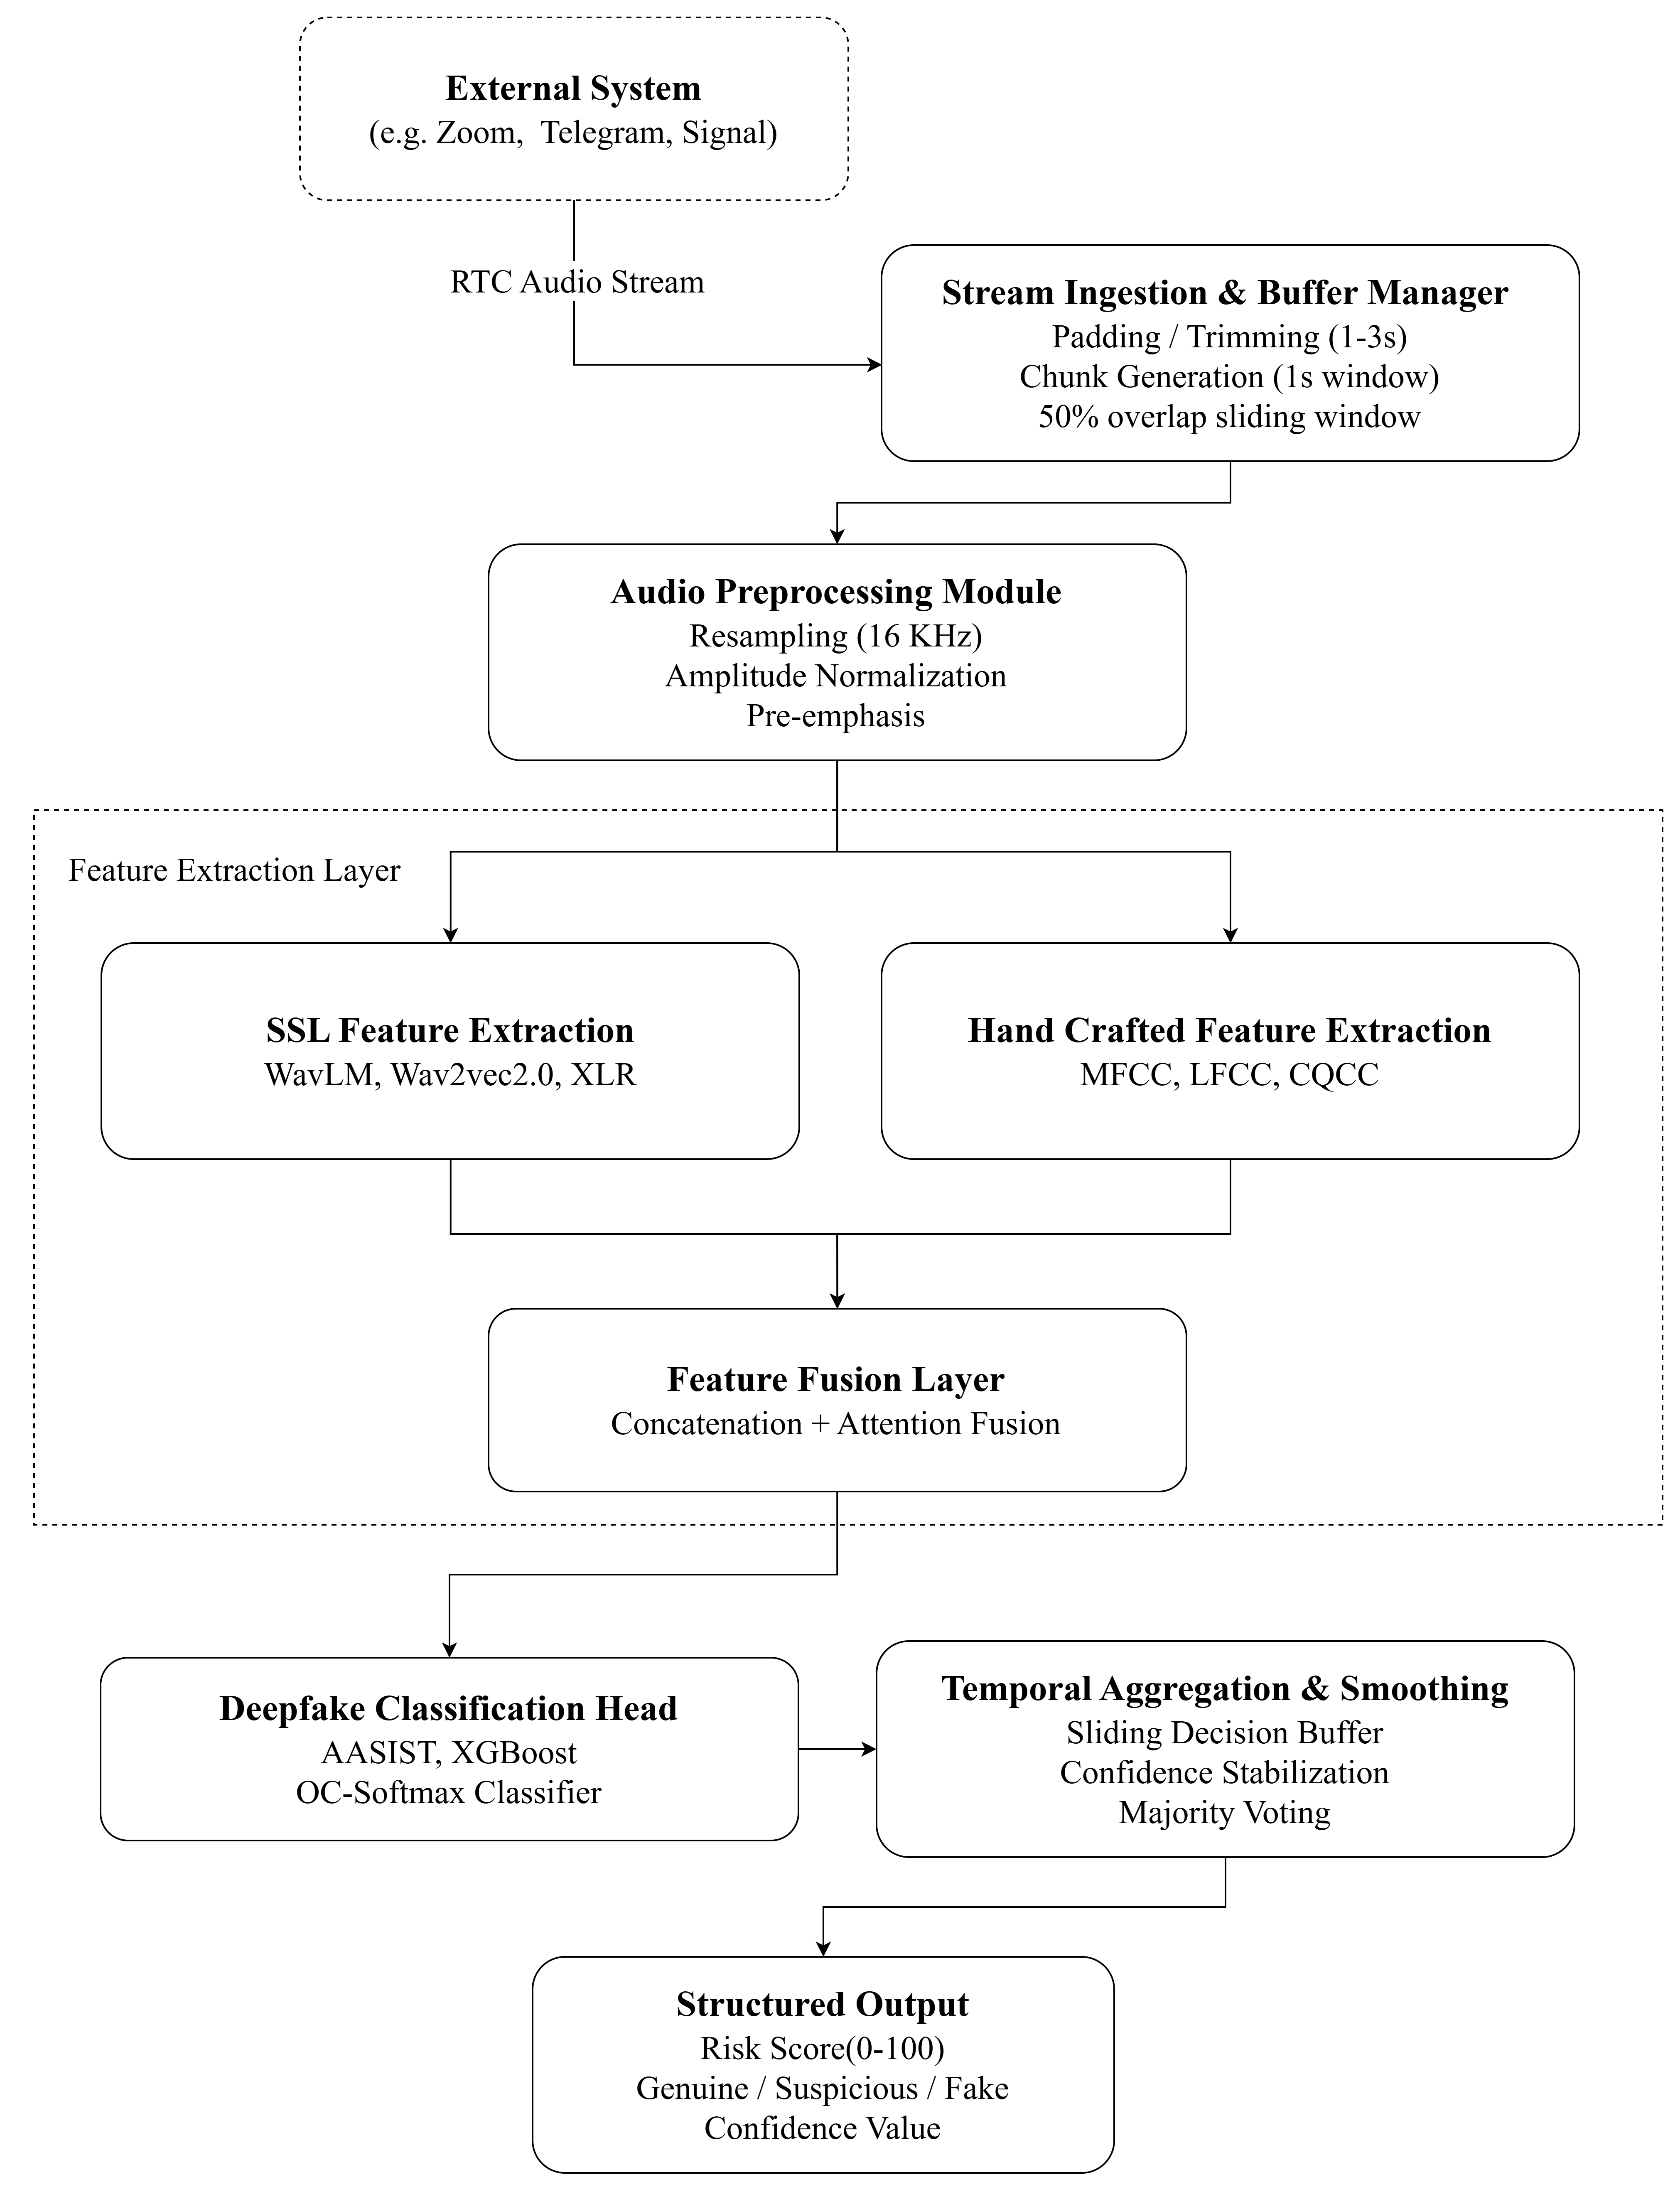
\includegraphics[width=1\textwidth]{images/methodology/detection_service.png}
    \vspace{0.25cm}
    \caption{Audio Deepfake Detection Service}
    \label{fig:detection_service}
\end{figure}

The audio deepfake detection service is the core inference component of the proposed system. It receives reconstructed receiver-side audio and performs analysis to determine whether the speech segment is real or synthetic. In contrast to tightly coupled end-to-end RTC implementations, the proposed design isolates deepfake detection as an independent service that can be integrated into different RTC/VoIP platforms through a standard API layer.

This service operates on short streaming windows rather than complete utterances, which makes it suitable for real-time deployment. Its output is a probabilistic decision that can be consumed by the RTC application for alert generation, monitoring, or downstream security enforcement.

\subsubsection{Service Architecture}

The detection module is implemented as a stateless inference service exposed through gRPC or HTTP APIs. This architecture allows the RTC system to send continuous stream to the detector without requiring modifications to the core communication stack.

Let the reconstructed receiver-side audio be denoted as $x_{out}[n]$.

The RTC client or receiver component forwards successive audio chunks to the detection service, which processes each chunk independently while preserving limited contextual information for temporal stability. The service can therefore be deployed in different environments, including:
\begin{itemize}
    \item centralized cloud servers,
    \item edge nodes close to the RTC application,
    \item embedded deployment within a monitored communication platform.
\end{itemize}

This separation improves modularity, scalability, and maintainability. It also allows the deepfake detector to be updated independently of the RTC transmission pipeline.

\subsubsection{Stream Ingestion and Buffer Manager}

Because RTC systems operate on continuous audio streams, the detection service processes audio in short overlapping windows rather than waiting for an entire conversation to complete. Let the incoming reconstructed stream be segmented into windows of length \(L\) with overlap \(O\).

The streaming input can be written as
\begin{equation}
X = \{x_1, x_2, \ldots, x_T\},
\end{equation}
where each \(x_t\) represents a short audio chunk extracted from \(x_{out}[n]\).

The chunking strategy serves two purposes:
\begin{itemize}
    \item It reduces inference latency by enabling online processing,
    \item It preserves local temporal context needed for reliable spoof detection.
\end{itemize}

Overlapping windows are used to reduce instability near chunk boundaries and to ensure that short-lived artifacts are not missed due to segmentation. In practice, the detector produces one prediction per chunk, and these predictions are later aggregated into a stable decision.

\subsubsection{Audio Preprocessing Module}

Before feature extraction, each input chunk is normalized and prepared for model inference. This preprocessing stage is lightweight and deterministic so that it does not introduce unnecessary latency.

Typical preprocessing operations include:
\begin{itemize}
    \item \textbf{Resampling} to a fixed sampling rate (16KHz) to match the training data.
    \item \textbf{Amplitude Normalization} standardizes the volume levels.
    \item \textbf{Pre-emphasis} applies a first order high-pass filter to amplify high frequency components.
    \item Trimming of silence or non-speech padding to mitigate variations caused by different microphones or sender side gain control,
    \item fixed-length padding for short segments.
\end{itemize}

Pre-emphasis is critical because RTC codecs often supress high frequencies yet these bands often contain the subtle spectral cues left by synthetic vocoders. 

The result is a standardized audio segment suitable for feature extraction:
\begin{equation}
\tilde{x}_t = P(x_t),
\end{equation}
where \(P(\cdot)\) denotes the preprocessing function and \(\tilde{x}_t\) is the normalized input chunk.

\subsubsection{Feature Extraction Pipeline}

The feature extraction stage converts the preprocessed waveform into representations that expose differences between real and synthetic speech. In the proposed framework, the system extracts two complementary views of audio simultaneously.

Let
\begin{equation}
z_t = F(\tilde{x}_t),
\end{equation}
where \(F(\cdot)\) denotes the feature extraction function and \(z_t\) is the resulting feature embedding.

The feature extraction module includes the following components:

\begin{itemize}

    \item \textbf{Hand-Crafted Acoustic Features:}
    Traditional acoustic descriptors are extracted to capture low-level spectral and temporal characteristics of speech. These features include Mel-Frequency Cepstral Coefficients (MFCCs), spectral centroid, spectral bandwidth, zero-crossing rate, short-time energy, and pitch-related descriptors. Such features provide information about frequency distribution, voice quality, and temporal variations that may reveal artifacts introduced by speech synthesis and vocoding systems.

    \item \textbf{Self-Supervised Speech Embeddings:}
    High-level contextual speech representations are extracted using pretrained self-supervised learning (SSL) models such as WavLM, or Wav2Vec~2.0. These models generate rich embeddings that capture long-range acoustic and linguistic information while remaining robust to noise, codec compression, and transmission distortions commonly observed in RTC environments.

    \item \textbf{Frame-Level Acoustic Representations:}
    The continuous speech signal is segmented into short analysis frames, and frame-level embeddings are generated for each segment. These representations preserve local spectral dynamics, temporal transitions, and fine-grained acoustic patterns that may contain artifacts associated with synthetic speech generation.

    \item \textbf{Phoneme-Aligned Feature Aggregation:}
    To improve linguistic consistency modeling, frame-level features are aggregated according to estimated phoneme boundaries. This process groups acoustically related frames into linguistically meaningful units, enabling the system to capture inconsistencies between phonetic content and acoustic realization that are often observed in deepfake speech.

\end{itemize}

By combining hand-crafted acoustic descriptors with self-supervised contextual representations, the proposed framework captures complementary information from both low-level signal characteristics and high-level speech structure.

Self-supervised embeddings are particularly useful because they capture high-level speech structure and remain relatively robust under codec compression, packet loss, and receiver-side enhancement. Phoneme-aligned aggregation further reduces sensitivity to frame-level noise by summarizing features over more stable linguistic units.

The detector is not relying solely on raw waveform patterns; it operates on representations that retain both acoustic detail and contextual speech information.

\subsubsection{Classification Model Design}

The classification module is responsible for determining whether a reconstructed RTC audio segment corresponds to real human speech or AI-generated synthetic speech. To evaluate both detection performance and real-time deployment feasibility, two complementary classification approaches are employed: AASIST and XGBoost.

For each incoming audio chunk $x_t$, a feature representation $z_t$ is first extracted through the feature extraction pipeline. The resulting representation is then forwarded to a classification model that estimates the probability that the observed speech segment is spoofed.

The classification process is defined as
\begin{equation}
s_t = \mathcal{C}(z_t),
\end{equation}
where $z_t$ denotes the extracted feature representation, $\mathcal{C}(\cdot)$ represents the classifier, and $s_t \in [0,1]$ is the spoofing probability assigned to audio chunk $t$.

\textbf{AASIST-Based Classification}

AASIST (Audio Anti-Spoofing using Integrated Spectro-Temporal Graph Attention Networks) serves as the primary deep learning detector in the proposed framework. Unlike conventional architectures that process temporal and spectral information separately, AASIST models speech as a heterogeneous graph and learns relationships between temporal and frequency-domain representations through graph attention mechanisms.

Given an input audio segment $x_t$, AASIST directly extracts discriminative spoofing representations and produces a spoofing score
\begin{equation}
s_t^{AASIST} = \mathcal{A}(x_t),
\end{equation}
where $\mathcal{A}(\cdot)$ denotes the AASIST network. The model learns artifacts introduced by Text-to-Speech (TTS), Voice Conversion (VC), and other speech synthesis techniques, making it highly effective for audio deepfake detection. Due to its state-of-the-art performance on ASVspoof benchmarks and relatively compact architecture, AASIST is selected as the primary detector for evaluating robustness under RTC-induced degradations such as codec compression, packet loss, jitter buffering, and packet loss concealment.

\textbf{XGBoost-Based Classification}

XGBoost (Extreme Gradient Boosting) is employed as a computationally efficient baseline model. Unlike AASIST, which operates directly on waveform representations, XGBoost utilizes handcrafted acoustic features extracted from reconstructed RTC audio streams.

For each audio chunk, feature vectors consisting of Mel-Frequency Cepstral Coefficients (MFCCs), spectral statistics, energy-related descriptors, and other acoustic characteristics are extracted and represented as
\begin{equation}
z_t = [f_1,f_2,\ldots,f_n].
\end{equation}
The feature vector is then provided to the XGBoost classifier:
\begin{equation}
s_t^{XGB} = \mathcal{X}(z_t),
\end{equation}
where $\mathcal{X}(\cdot)$ denotes the trained XGBoost model. The classifier generates a spoofing probability based on an ensemble of gradient-boosted decision trees.

XGBoost is included because previous studies have demonstrated that it achieves strong detection performance while maintaining extremely low inference latency. Consequently, it provides an effective benchmark for assessing the trade-off between detection accuracy and real-time computational efficiency.

\subsubsection{Temporal Aggregation and Decision Stabilization}

Since inference is performed on successive streaming chunks, individual predictions may fluctuate due to short-term artifacts, transient packet loss, or local noise variation. To improve decision stability, the proposed system applies temporal aggregation over a sliding window of recent predictions.

Let the set of recent spoofing scores be
\begin{equation}
S_t = \{s_{t-k+1}, s_{t-k+2}, \ldots, s_t\},
\end{equation}
where \(k\) is the aggregation window size.

A smoothed score can be computed as
\begin{equation}
\bar{s}_t = A(S_t),
\end{equation}
where $A(\cdot)$ denotes the aggregation function. In implementation, this may be a moving average, weighted average, or majority-based smoothing rule.

The final decision is then obtained from the aggregated score:
\begin{equation}
\hat{d}_t =
\begin{cases}
1, & \bar{s}_t \geq \tau \\
0, & \bar{s}_t < \tau
\end{cases}
\end{equation}

This stabilization step reduces false alarms caused by isolated distortions and produces a more reliable real-time output for the RTC application.

\subsubsection{Output Interface and Response Format}

The detection service returns a structured output to the RTC system through the same API channel used for audio ingestion. The response contains both a continuous risk score and a discrete decision label.

A typical output contains:
\begin{itemize}
    \item spoofing probability score \(s_t\),
    \item binary class label \(\hat{d}_t\),
    \item optional confidence value,
    \item optional timestamp or chunk identifier.
\end{itemize}

The output can therefore be represented as
\begin{equation}
R_t = \{s_t, \hat{d}_t, \text{timestamp}_t\}.
\end{equation}

This response enables real-time actions such as UI alerts, call monitoring warnings, logging for security analysis, and policy-based intervention by the RTC platform.